\documentclass[11pt]{beamer}

\usepackage{physics, amsmath, amssymb, mathtools, latexsym, amsfonts, scalefnt}
\usepackage{tikz, lipsum, lmodern, wrapfig, svg, subcaption}
\usepackage[backend=biber, style=alphabetic]{biblatex}
\usepackage[most]{tcolorbox}
\usepackage{epigraph}
\usepackage{macros-beamer}
\usepackage{silence}
\WarningFilter{latexfont}{}
\usetikzlibrary{positioning, shapes.geometric, arrows.meta}

\usetheme{Madrid}
% \usecolortheme{orchid}
\usecolortheme{whale}

\title[LSR Bounds for Networked Systems]
{Bounds of Validity for Bifurcations of Equilibria in a Class of Networked Dynamical Systems}

\subtitle{American Control Conference, 2026}

\author
[
    \textcolor{yellow}{Pranav~Gupta} \and
    R.~Banavar \and
    A.~Bizyaeva
]
{
    \alert{P.~Gupta \inst{1}}   \and
    R.~Banavar      \inst{1}    \and
    A.~Bizyaeva     \inst{2}
}

\institute[]
{
    \inst{1}
    Indian Institute of Technology Bombay\and
    \inst{2}
    Cornell University
}

\date{May 29, 2026}

\addbibresource{ref.bib}

\begin{document}

\maketitle

\begin{frame}{Contents}
    \tableofcontents
\end{frame}

\section{Bifurcations and Networked Systems}

\subsection{Introduction to Bifurcations}

\begin{frame}{Introduction to Bifurcations}
    \begin{block}{Definition}
        Topological changes in the flow (equilibria, stability, oscillations, chaos) when system parameter(s) cross a threshold are called \textbf{bifurcations}.
    \end{block}
    \begin{figure}[ht!]
        \centering
        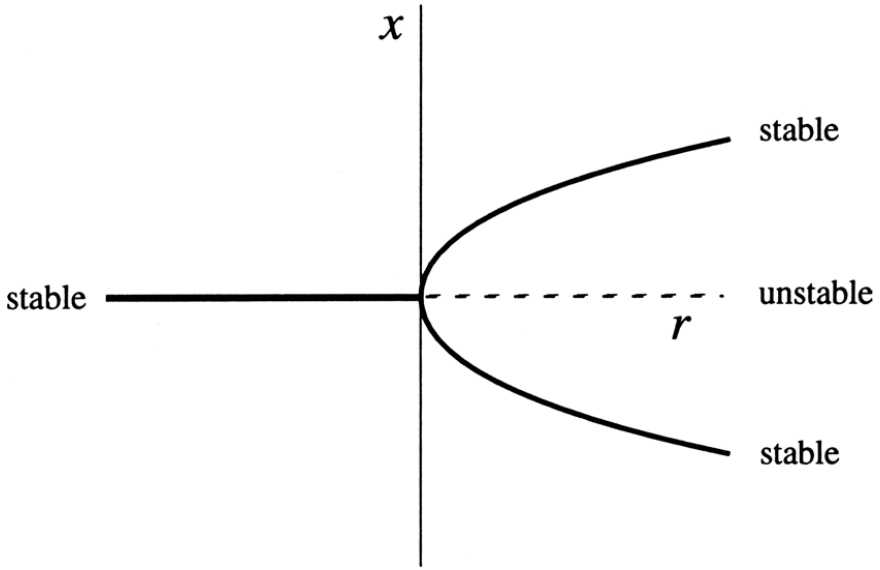
\includegraphics[height=40mm]{images/super-pitch.png}
        \caption{pitchfork bifurcation diagram for \(\dot{x}=rx-x^{3}\).}
    \end{figure}
    % \begin{columns}
    %     \begin{column}{0.33\textwidth}
    %         \begin{figure}[ht!]
    %             \centering
    %             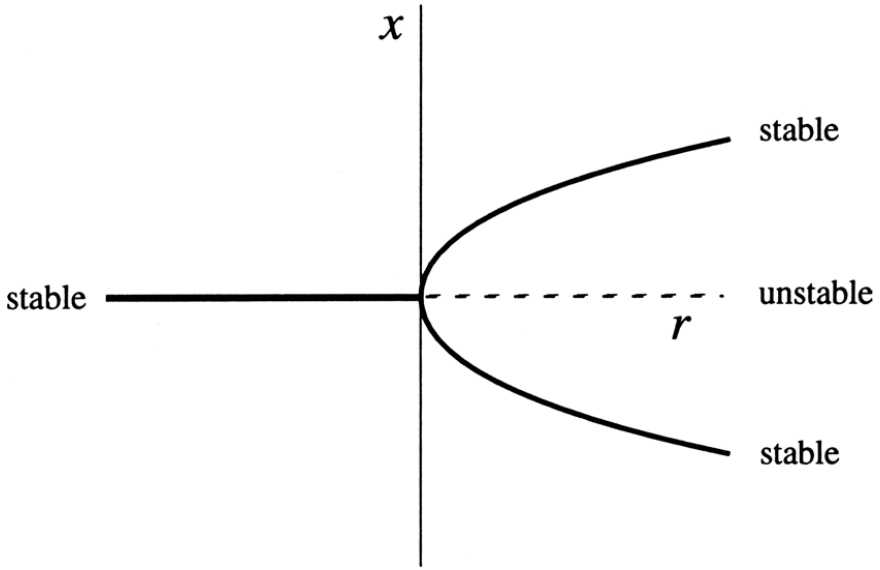
\includegraphics[width=0.75\textwidth]{images/super-pitch.png}
    %             \caption{pitchfork bifurcation diagram}
    %         \end{figure}
    %     \end{column}
    %     \begin{column}{0.7\textwidth}
    %         \(\dot{x}=rx-x^{3}\)
    %         \begin{itemize}
    %             \item \(r<0\implies\) stable f.p. at \(x^{\star}=0\)
    %             \item \(r_{c}=0\implies\) weakly stable f.p. at \(x^{\star}=0\)
    %             \item \(r>0\implies\begin{cases}
    %                       \text{stable f.p. at } x^{\star}=\pm\sqrt{r} \\
    %                       \text{unstable f.p. at } x^{\star}=0
    %                   \end{cases}\)
    %         \end{itemize}
    %     \end{column}
    % \end{columns}
\end{frame}

\subsection{Bifurcations in Networked Systems}

\begin{frame}{Bifurcations in Networked Systems}
    Many real-world networked systems exhibit \emph{sudden qualitative shifts} in behaviour, which can be modelled as bifurcations:
    \begin{itemize}
        \item \textbf{Opinion dynamics}: a population suddenly reaching consensus
        \item \textbf{Network epidemics}: transition from disease-free to endemic state
        \item \textbf{Gene regulatory networks}: switching between cell states
    \end{itemize}

    \vspace{5mm} \pause

    The \alert{\LSR{}} used to predict and engineer these shifts, but it is inherently local with the validity region typically unknown.

    \vspace{3mm}

    \begin{center}
        \emph{How far from the bifurcation point can we trust the reduction?}
    \end{center}
\end{frame}

\subsection{Hopfield and Firing Rate Models}

\begin{frame}{Hopfield and Firing Rate Models}
    \setlength{\abovedisplayskip}{3pt}
    \setlength{\belowdisplayskip}{3pt}
    \setlength{\jot}{1pt}

    \begin{block}{System Definition}
        We study nonlinear network systems of the form:
        \begin{subequations}
            \begin{align}
                \textbf{Hopfield}:    \dot{x} & = \Psi(x,p) = -Cx + pAS(x) + b \\
                \textbf{Firing Rate}: \dot{x} & = \Psi(x,p) = -Cx + S(pAx + b)
            \end{align} \label{NDS}
        \end{subequations}
        with constant \alert{bias} \(b\), \alert{adjacency} matrix \(A\), diagonal \alert{dissipation} matrix \(C \succ 0\), nonlinear element-wise \alert{activation} \(S(z) = [S_1(z_1), \dots, S_n(z_n)]^{\top}\).
        Standard assumptions made about the existence of a bifurcation point, and non-degeneracy in eigenvalues of jacobian \(J=D_{x}\Psi(x^{\star},p^{\star})\).
    \end{block}

    \vspace{4mm} \pause

    \textbf{Applications}: modelling of \emph{dynamic neural networks}, \emph{opinion dynamics}, \emph{Lur'e feedback systems}, \emph{gene regulatory networks}, etc.

    \vspace{4mm} \pause

    \textbf{Objective}: derive \alert{explicit bounds} for the validity region of the LSR for these two classes of models.
\end{frame}

\section{\LSR{} and Explicit Bounds}

\subsection{Introduction}

\begin{frame}{\LSR{}: introduction}
    \begin{block}{\LSR{}}
        \begin{itemize}
            \item Bifurcations in high-dimensional systems typically occur on low-dimensional \alert{centre manifold}.
            \item \textbf{L.S. Reduction}: projecting dynamics onto lower-dimensional critical subspace at bifurcation points; \alert{preserves local topological equivalence}.
            \item \textbf{Advantage}: \emph{no explicit centre manifold computation}; direct use of singularity-theoretic tools \cite{Golubitsky1985}.
        \end{itemize}
    \end{block}

    \vspace{4mm} \pause

    \textbf{Output}: reduced algebraic system with bifurcation diagram \alert{locally isomorphic} to original system \emph{(equilibria in bijective correspondence)}.
\end{frame}

\subsection{Overview of Algorithm}

\begin{frame}{\LSR{}: overview of algorithm}
    \begin{columns}
        \vspace{-8mm}
        \begin{column}{0.45\textwidth}
            \begin{itemize}
                \itemsep 0em
                \scalefont{0.75}
                \item Smooth NLTI system \(\dot{\mathbf{x}}=\boldsymbol{\Phi}(\mathbf{x},\lambda)\)
                \item Singular point at \((\mathbf{x}^{\star},\lambda^{\star})\):
                      \begin{itemize}
                          \scalefont{0.75}
                          \item \(\boldsymbol{\Phi}(\mathbf{x}^{\star},\lambda^{\star}) = 0\)
                          \item For \(J=D_{x}\Phi(\mathbf{x}^{\star},\lambda^{\star})\), \(q:=\dim\big(\mathrm{ker}(J)\big)>0\)
                      \end{itemize}
                \item Linear orthogonal projection operator \(P:\R[n]\to\mathrm{range}(J)\)
            \end{itemize}
            \begin{figure}[ht!]
                \centering
                \includesvg[width=.9\textwidth]{images/LSR.svg}
                \caption{sketch of LSR for a \(2-\dim\) system with a pitchfork bifurcation}
            \end{figure}
        \end{column}
        ~
        \begin{column}{0.55\textwidth}
            \begin{tikzpicture}[node distance=1cm]
                \node (state) [startstop] {decompose \(x \in X\) into coords \\ \(\alpha \in \R[q]\) along \(\ker(J)\) and \\ \(\beta \in \R[n-q]\) along \(\ker(J)^{\perp}\)};
                \node (Phi) [process, below of=state, yshift=-3mm] {decompose \(\{\Phi=0\}\) \\ into components};
                \node (perp) [process, below of=Phi, xshift=-20mm] {\(\{(I-P)\Phi=0\}\) \\ along \(\range(J)^{\perp}\)};
                \node (para) [process, right of=perp, xshift=30mm] {\(\{P\Phi=0\}\) \\ along \(\range(J)\)};
                \node (elim) [decision, below of=perp, yshift=-7mm] {eliminate \(\beta\) \\ dependence};
                \node (imft) [process, below of=para, yshift=-7mm] {apply ImFT \\ \((\alpha, \lambda)  \mapsto \beta\)};
                \node (project) [process, below of=elim, xshift=20mm, yshift=-2mm] {obtain \(\phi : \R[q] \times \R[m] \to \R[n]\)};
                \node (voila) [startstop, below of=project, yshift=-3mm] {obtain reduced \(q-\)dim rep \\ \(\varphi : \R[q] \times \R[m] \to \R[q]\)};

                \draw [arrow] (state) -- (Phi);
                \draw [arrow] (Phi) -| (perp);
                \draw [arrow] (Phi) -| (para);
                \draw [arrow] (perp) -- (elim);
                \draw [arrow] (para) -- node[midway, align=center, yshift=1mm] {\tiny \(J : \ker(J)^{\perp} \to \range(J)\) \\[-2mm] \tiny is an invertible operator} (imft);
                \draw [arrow] (imft) -- node[midway, above] {\tiny substitute} (elim);
                \draw [arrow] (elim) -- (project);
                \draw [arrow] (project) -- node[midway, align=center, yshift=1mm] {\tiny project onto \(\range(J)^{\perp}\;\,\)} (voila);
            \end{tikzpicture}
        \end{column}
    \end{columns}
\end{frame}

\subsection{Explicit Bounds on \ImFT{}}

\begin{frame}{\ImFT{} and Bounds}

    \setlength{\abovedisplayskip}{3pt}
    \setlength{\belowdisplayskip}{3pt}
    \setlength{\jot}{1pt}

    \begin{block}{\ImFT{}}
        System \(f(u,v)=f(u_0,v_0)\) with invertible linearisation \(D_{v}f(u_0,v_0)\) has a \textit{local unique smooth implicit representation} \(v=g(u)\) near \((u_0,v_0)\).
    \end{block} \pause
    \begin{block}{Theorem on Bounds for ImFT}
        Restating from \cite[Corollary 3.8]{jindal2024estimates}, define the following quantities:
        \begin{itemize}
            \item \(M_{u} := \norm{D_{u}f(u_0,v_0)}\) and \(M_{v} := \norm{\big(D_{v}f(u_0,v_0)\big)^{-1}}\)
            \item \(L_u(r_u) := \sup_{u\in\mathcal{B}(u_0,r_u)} \norm{D_{u}f(u,v_0)-D_{u}f(u_0,v_0)}\)
            \item \(L_v(r_u,r_v) := \sup_{(u,v)\in\mathcal{B}(u_0,r_u)\times\mathcal{B}(v_0,r_v)} \norm{D_{v}f(u,v)-D_{u}f(u_0,v_0)}\)
        \end{itemize} \pause
        Then, for all \(r_u,r_v>0\) simultaneously satisfying
        \begin{equation*}
            L_{u}(r_u)r_u + L_{v}(r_u,r_v)r_v < \frac{r_v}{M_v} - M_ur_u
        \end{equation*}
        The implicit map \(g\) is \(\mathcal{C}^{1}\) and valid over \(g:\mathcal{B}(u_0,r_u)\to\mathcal{B}(v_0,r_v)\).
    \end{block}
\end{frame}

\subsection{Explicit Bounds on \LSR{}}

\begin{frame}{\LSR{}: explicit bounds}

    \setlength{\abovedisplayskip}{3pt}
    \setlength{\belowdisplayskip}{3pt}
    \setlength{\jot}{1pt}

    \begin{block}{Theorem on Bounds for LSR \cite{gupta2024estimates}}
        Let \(M_u, M_v, r_u, r_v, L_u, L_v \to \Mpr, \Mpp, \rpr, \rpp, L_{\parallel}, L_{\perp}\) denote the recasts of corresponding quantities into the \LSR{} framework. \\[3mm]
        Then, for all \(\rpr,\rpp > 0\) simultaneously satisfying
        \begin{equation*}
            \Lpr \rpr + \Lpp \rpp < \frac{\rpp}{\Mpp} - \Mpr \rpr
        \end{equation*}
        the implicit map \((\alpha,\lambda)\xmapsto{\varphi}\beta\) is valid over \(\varphi:\mathcal{B}\big((\alpha_0,\lambda_0),\rpr\big)\to\mathcal{B}\big(\beta_0,\rpp\big)\).
    \end{block}
    \begin{center}
        \vspace{4mm} \pause
        \emph{Derivations of LSR validity bounds for the general Hopfield and Firing Rate networked models \eqref{NDS} are presented in the accompanying paper.}

        \vspace{4mm} \pause
        We now apply these bounds to \alert{indecision-breaking bifurcations on regular graphs}, which canonically model \emph{consensus formation in opinion dynamics}.
    \end{center}

\end{frame}

\section{Application to Indecision-Breaking Consensus bifurcations}

\begin{frame}{NLOD Consensus Bifurcations: system}
    Consider the unbiased case for a \(k-\)regular graph:
    \begin{subequations}
        \begin{align}
            \textbf{Hopfield}:    \dot{x} & = -dx + uA\tanh(x) \\[-1pt]
            \textbf{Firing Rate}: \dot{x} & = -dx + \tanh(uAx)
        \end{align} \label{regular}
    \end{subequations}
    In both models, origin eqbm undergoes pitchfork bifurcation at \(u^{\star} = \tfrac{d}{k}\).
    
    \begin{figure}[ht!]
        \centering
        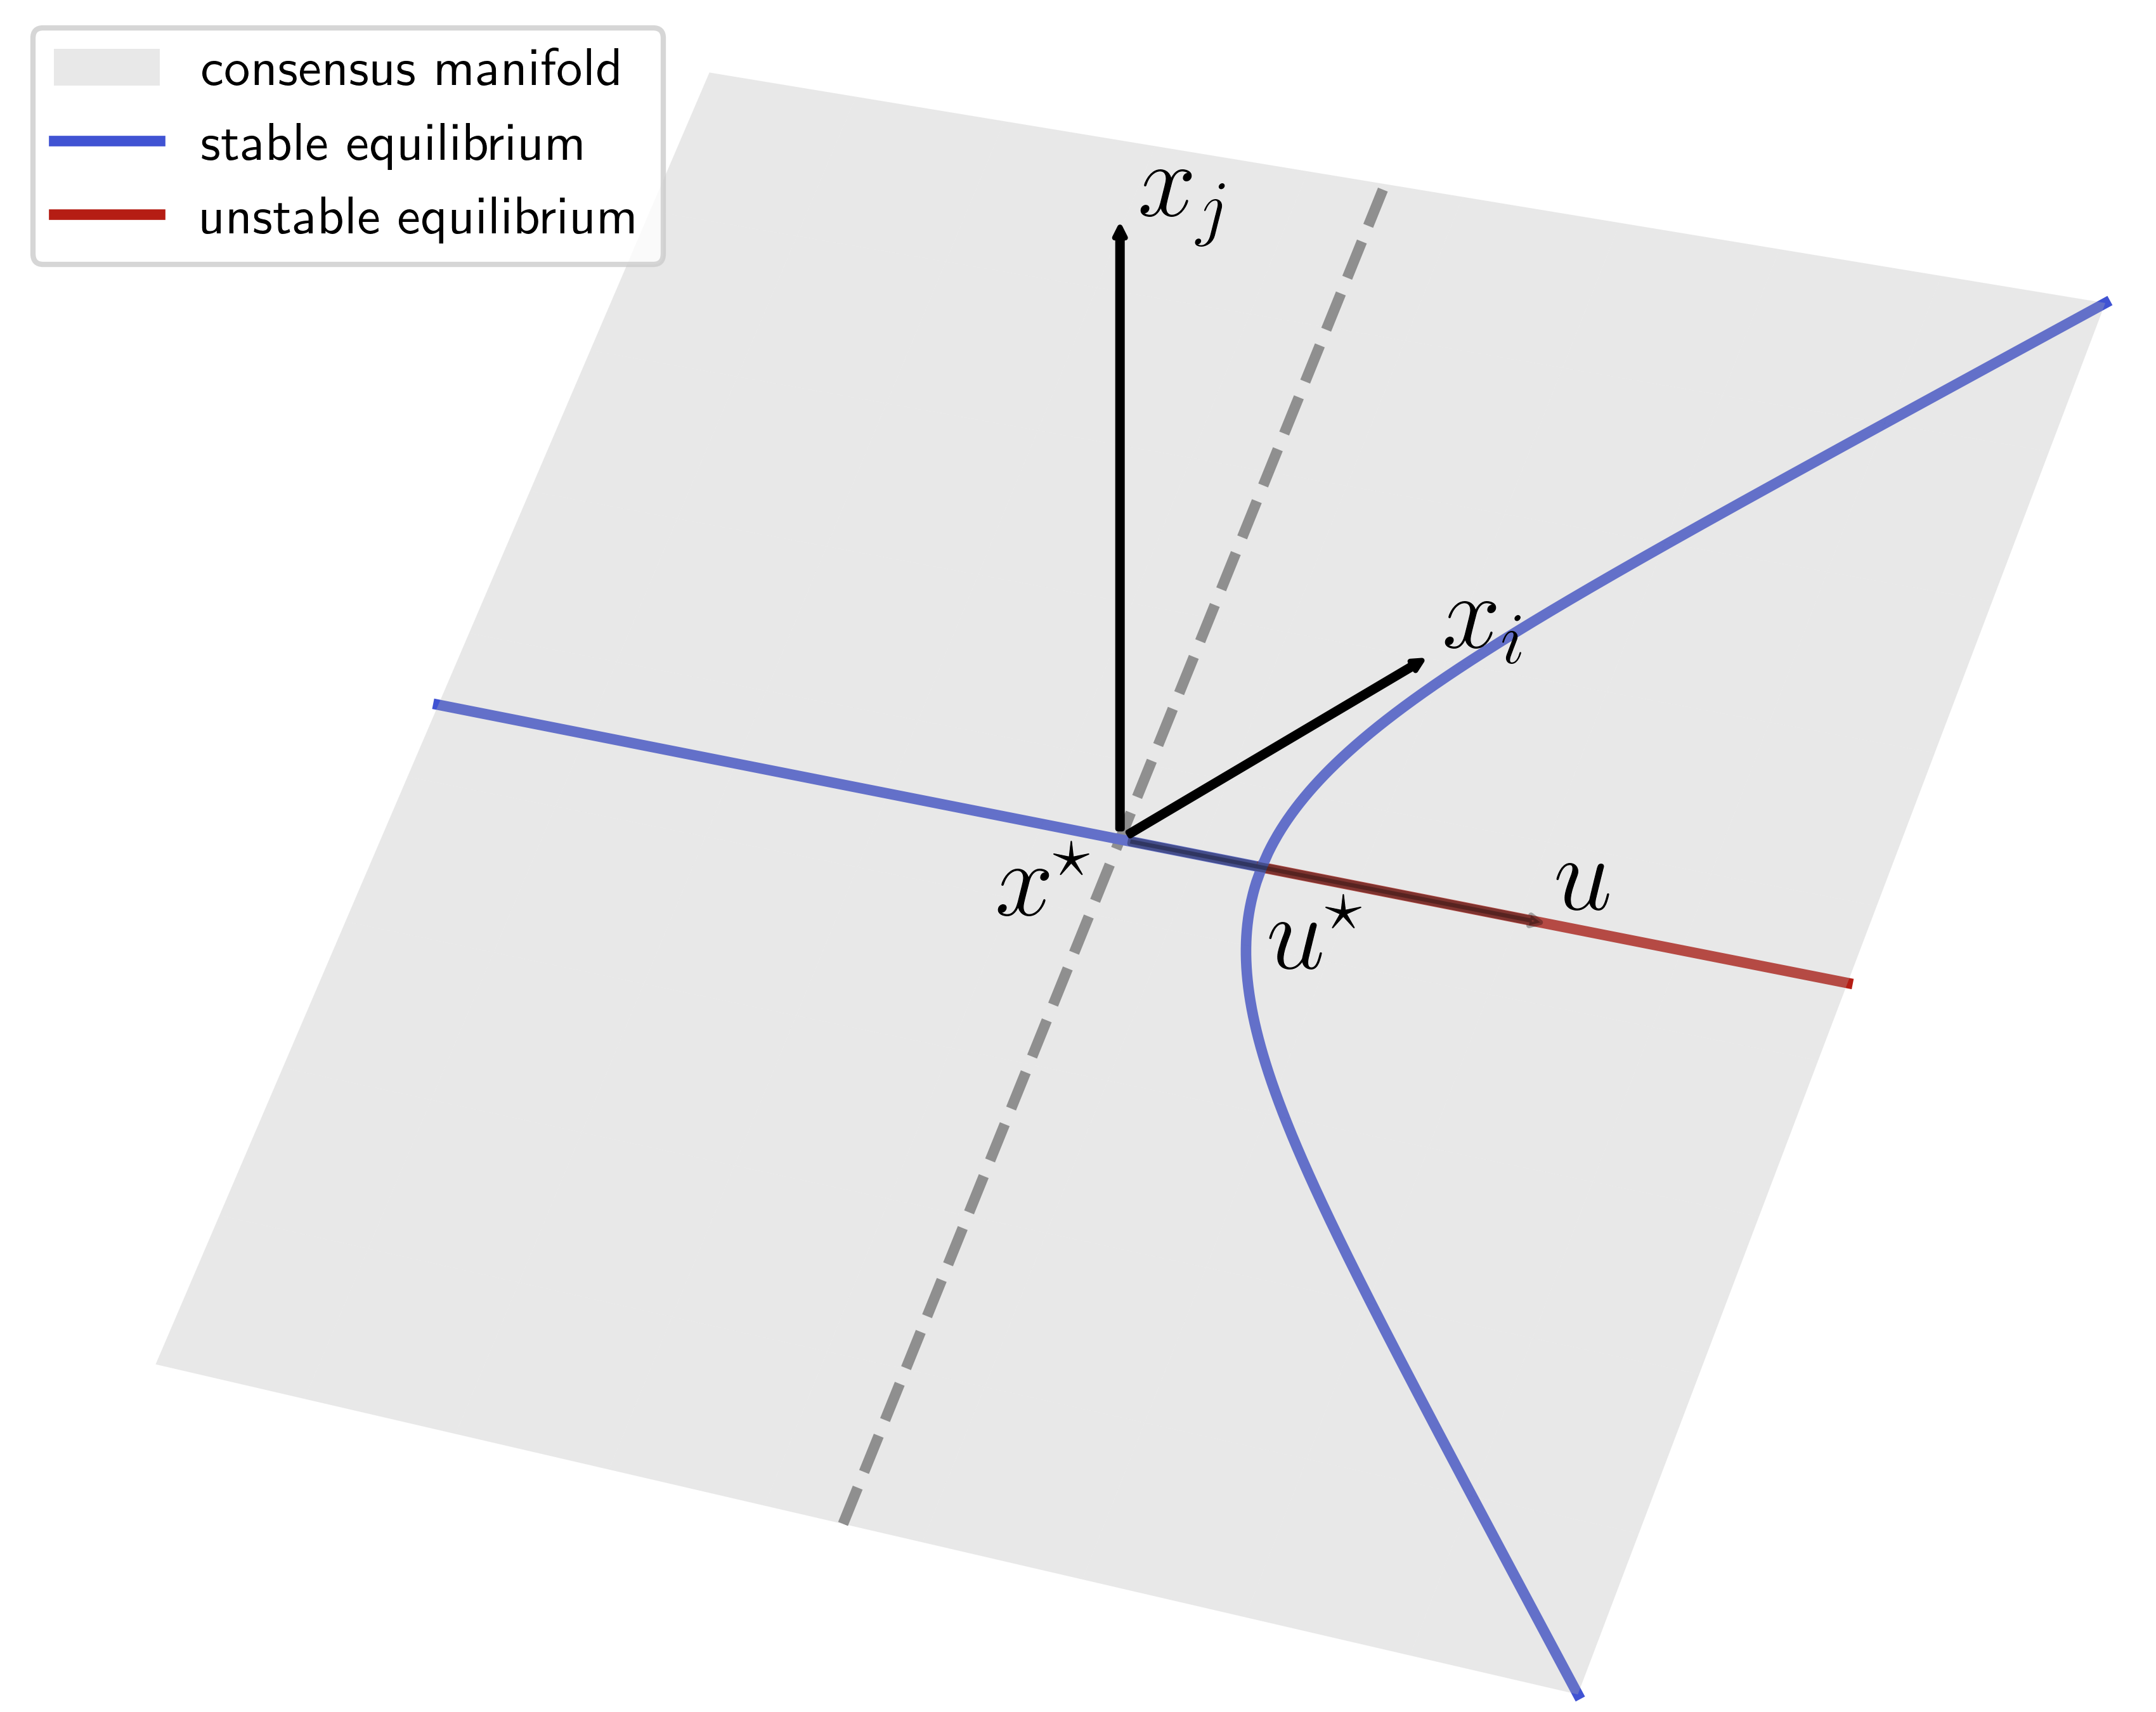
\includegraphics[height=40mm]{images/consensus.png}
        \caption{indecision-breaking bifurcation in \eqref{regular} at \((x^{\star},u^{\star})=\left(\mathbf{0}, \tfrac{d}{k}\right)\).}
    \end{figure}
\end{frame}

\begin{frame}{NLOD Consensus Bifurcations: bounds}
    \begin{block}{LSR Validity Bounds for NLOD Consensus Bifurcation}
        Bounds of LSR validity for the above bifurcation are given by
        \begin{itemize}
            \itemsep 0mm
            \item \(0<\rpr<\tfrac{d(k-\lambda_{2}(A))}{k\abs{\lambda'(A)}}\) \alert{along} consensus manifold
            \item \(\rpp>0\) \alert{normal} to consensus manifold
        \end{itemize}
        where \(k=\lambda_{1}(A) \ge \lambda_{2}(A) \ge \dots\) and \(\abs{\lambda'(A)} := \max_{i \neq 1}\{\abs{\lambda_{i}(A)}\}\).
    \end{block}

    \begin{columns}
        \begin{column}{.5\linewidth}
            \begin{figure}[ht!]
                \centering
                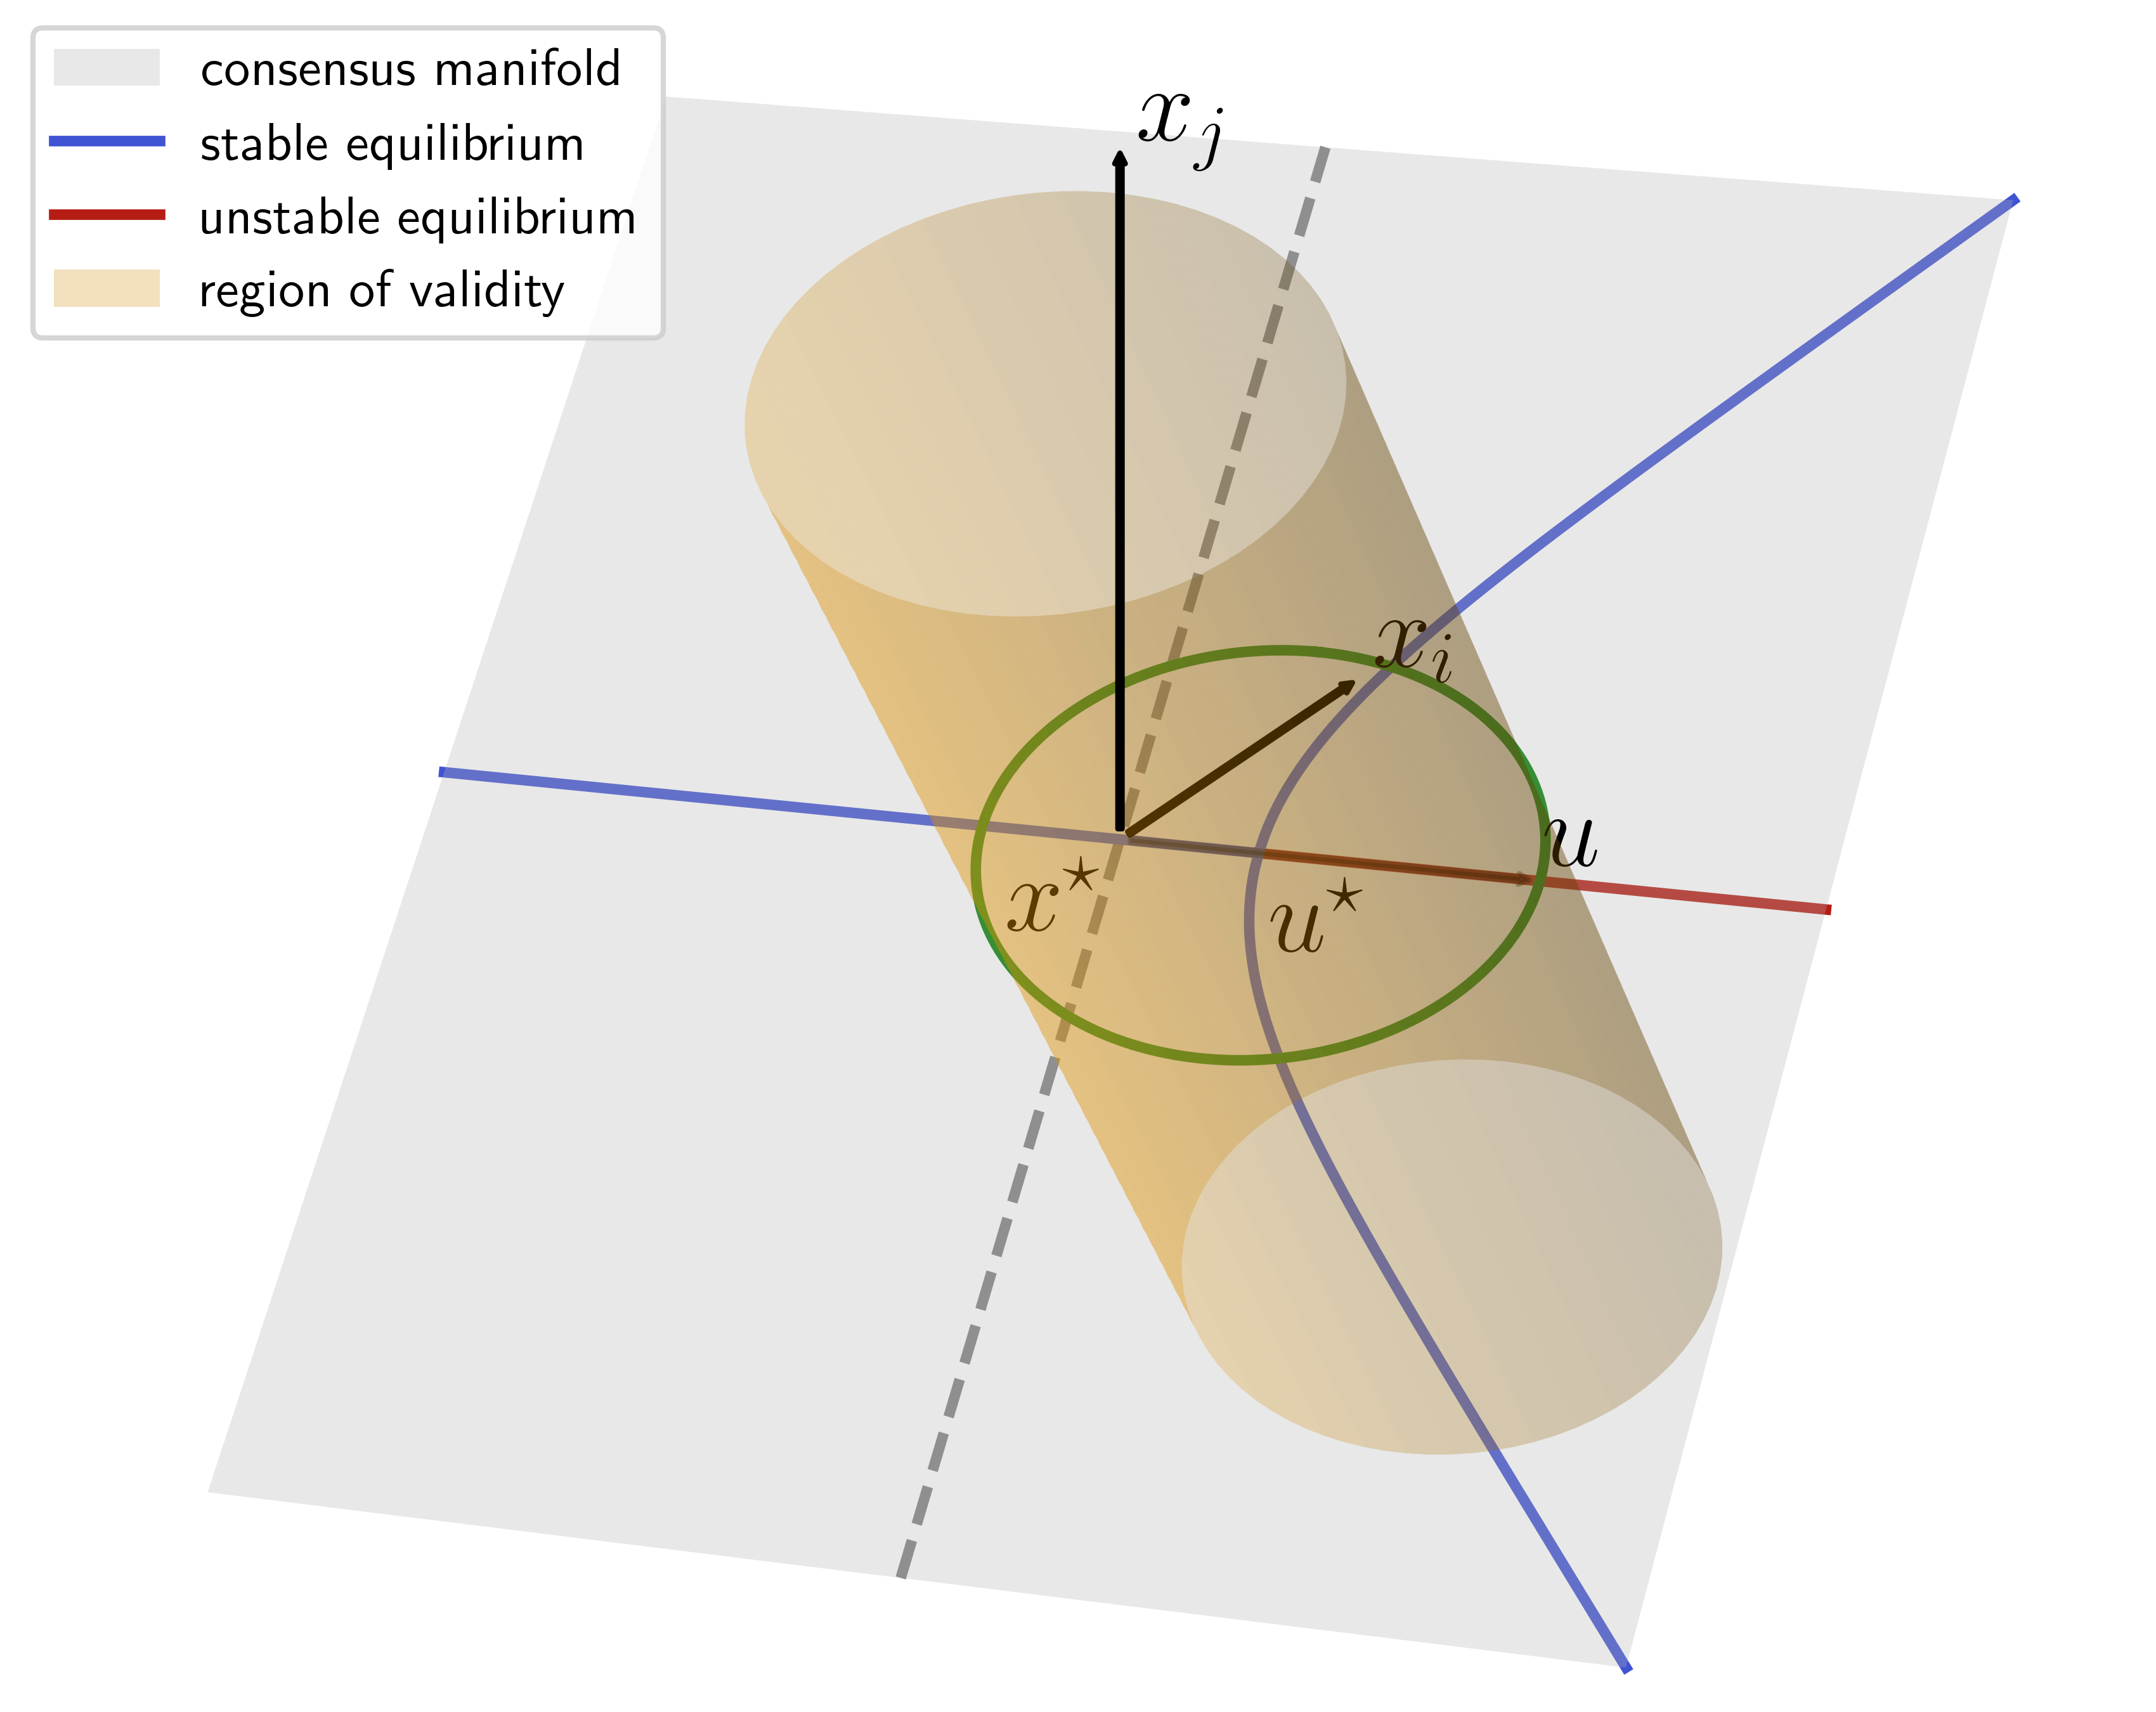
\includegraphics[height=36mm]{images/bounds.png}
                \caption{region of validity of LSR for \eqref{regular}.}
            \end{figure}
        \end{column}
        \pause
        \begin{column}{.5\linewidth}
            \textbf{Complete Graph}: bounds simplify to \(0<\rpr<\tfrac{dn}{n-1}\) and \(\rpp>0\) for the all-to-all complete \(n-\)graph case.
        \end{column}
    \end{columns}
\end{frame}

\begin{frame}{NLOD Consensus Bifurcations (plots)}
    \begin{figure}[ht!]
        \centering
        \captionsetup{justification=centering}
        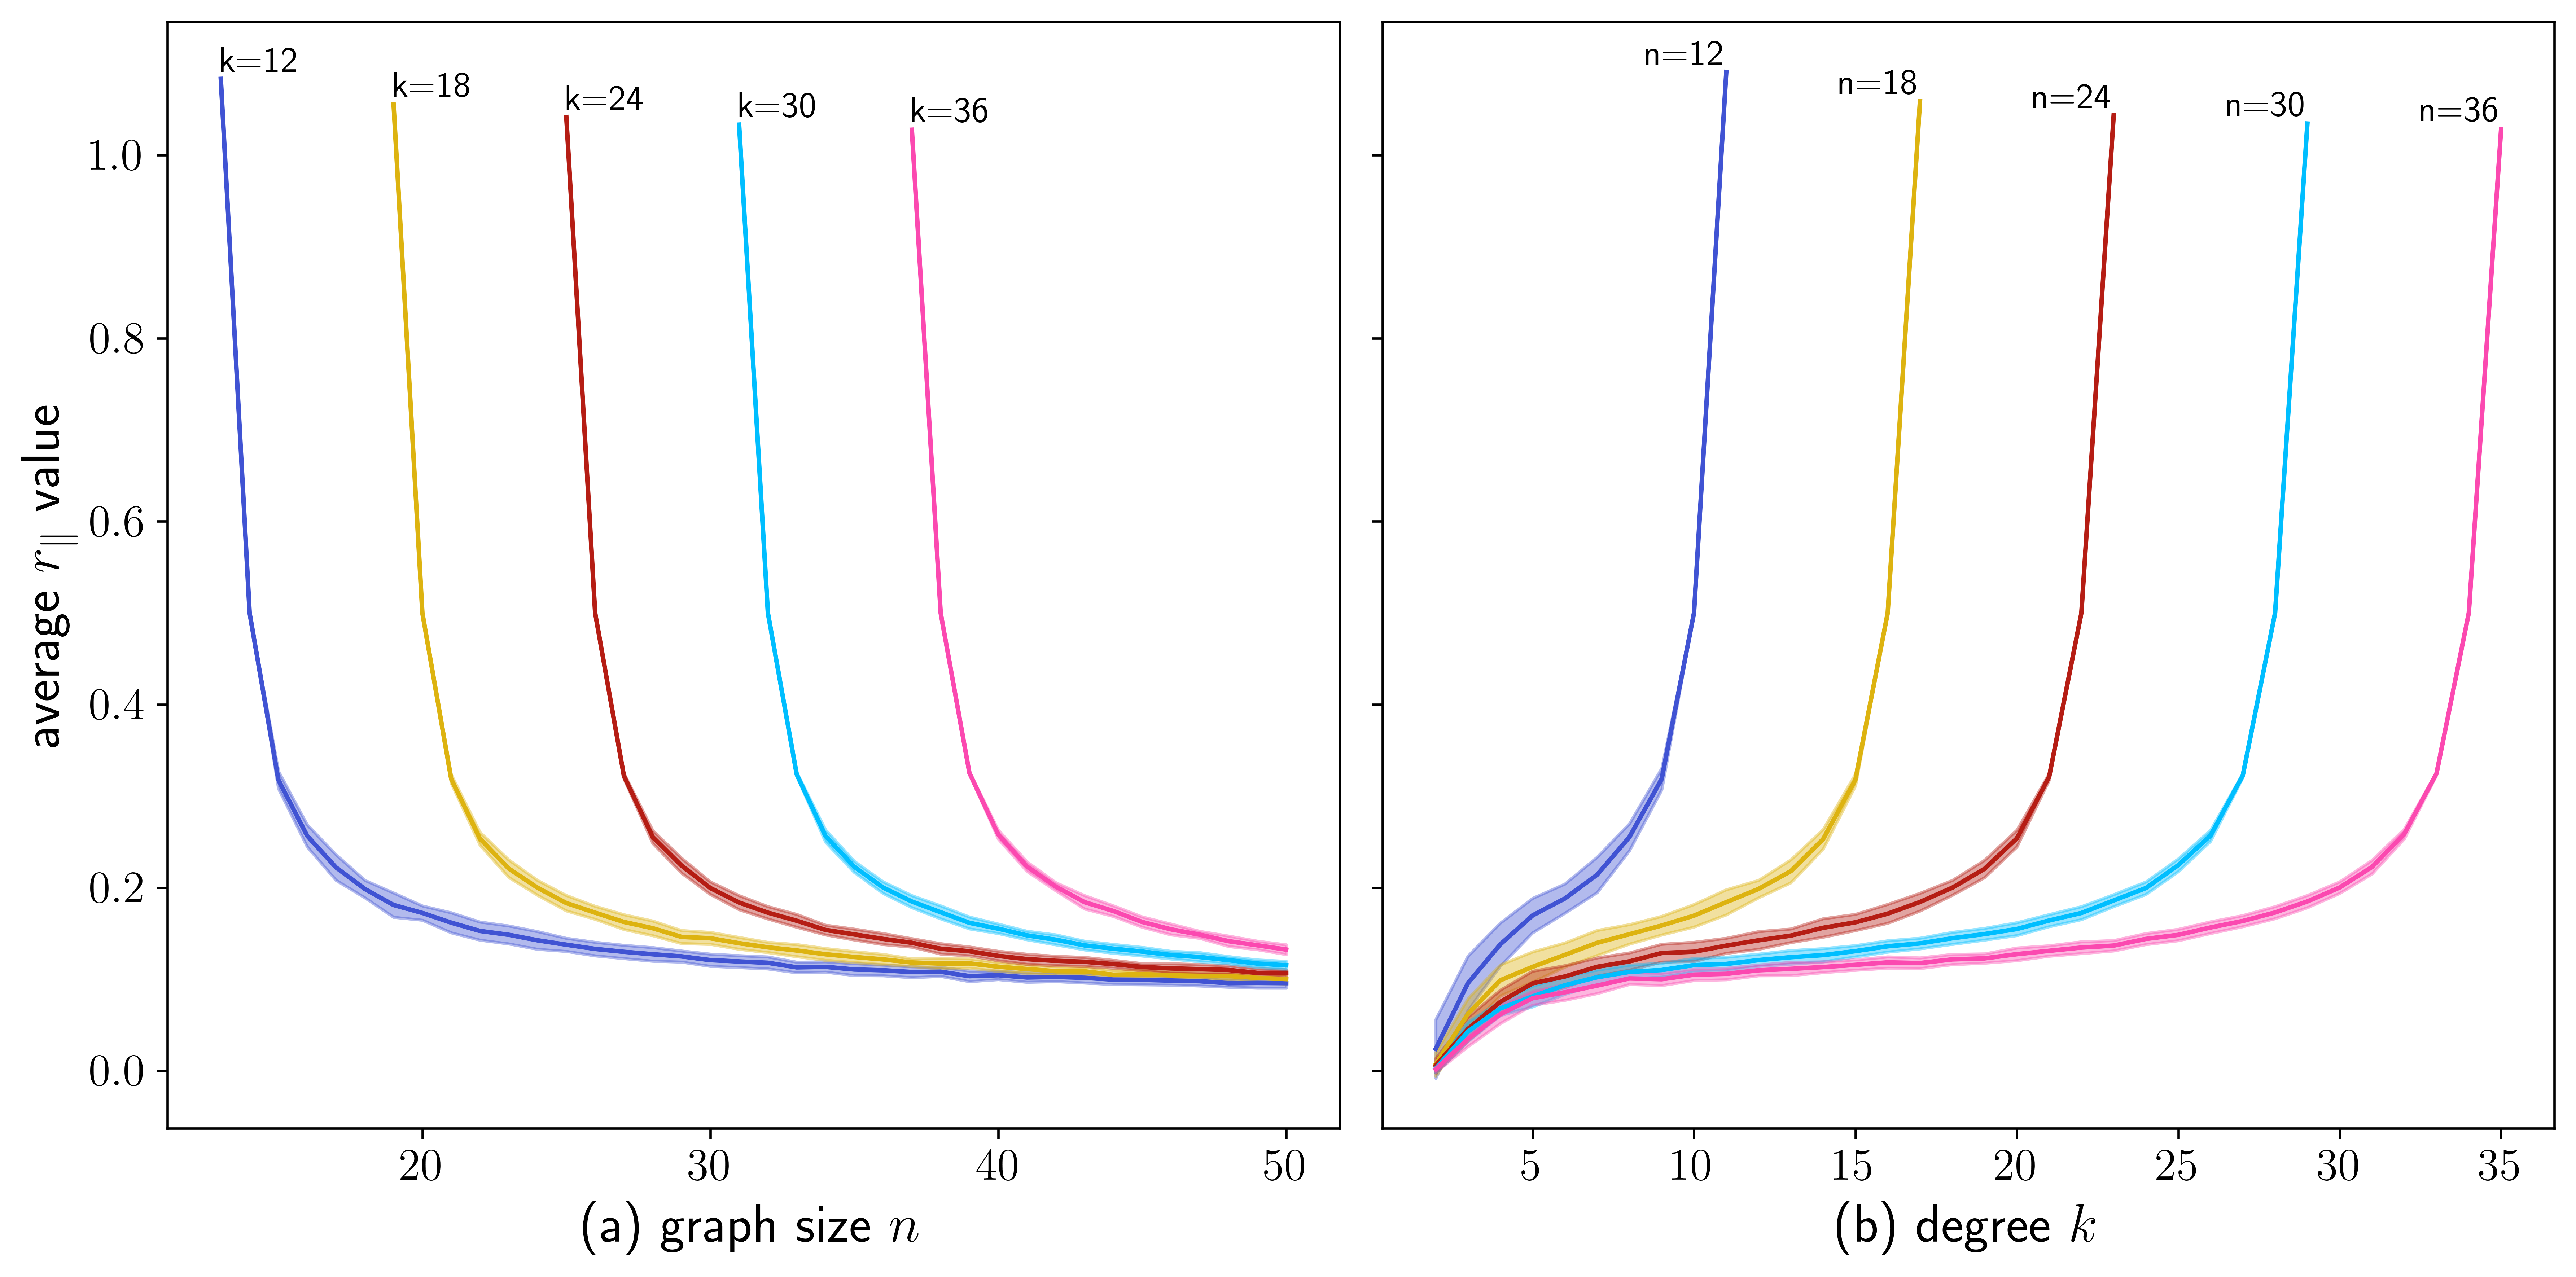
\includegraphics[width=0.8\linewidth]{images/regular-n-k.png}
        \caption{variation in bounds for NLOD over regular graphs (d=1): \\
            (a) fixed degree \(k\in\{12,18,24,30,36\}\), varying graph size \(n\).\\
            (b) fixed graph size \(n\in\{12,18,24,30,36\}\), varying degree \(k\).}
        \label{fig:nk_dependence}
    \end{figure}
\end{frame}

\section{Contributions}

\begin{frame}{Summary of Contributions}
    \begin{enumerate}
        \item Developed computable first-order bounds for the region where LSR analysis remains faithful to the full system by leveraging explicit bounds on ImFT to obtain explicit neighbourhood radii \((\rpr, \rpp)\).
        \item Specialized general bounds to two broad nonlinear network models:
              \begin{itemize}
                  \item Hopfield-type dynamics: \(\dot{x} = -Cx + pA S(x) + b\)
                  \item Firing rate-type dynamics: \(\dot{x} = -Cx + S(pAx + b)\)
              \end{itemize}
        \item Applied bounds to indecision-breaking pitchfork bifurcations on consensus dynamics over \(k-\)regular graphs, revealing dependence on:
              \begin{itemize}
                  \item graph size \(n\),
                  \item network degree \(k\),
                  \item spectral structure of \(A\).
              \end{itemize}
        \item Showed that Hopfield and Firing Rate NLOD yield \emph{identical} validity bounds over regular graphs due to shared local Jacobian structure.
    \end{enumerate}
\end{frame}

\begin{frame}{Thank You!}
    \begin{columns}[c]
        \column{0.32\textwidth}
        \centering
        
\includegraphics[height=3.5cm]{images/Pranav.jpg}

        \vspace{0.2cm}
        \textbf{Pranav Gupta}
        \small
        guptapranav@iitb.ac.in

        \column{0.32\textwidth}
        \centering
        
\includegraphics[height=3.5cm]{images/Ravi.jpg}

        \vspace{0.2cm}
        \textbf{Ravi Banavar}
        \small
        banavar@iitb.ac.in

        \column{0.32\textwidth}
        \centering
        
\includegraphics[height=3.5cm]{images/Anastasia.png}

        \vspace{0.2cm}
        \textbf{Anastasia Bizyaeva}
        \small
        asb379@cornell.edu
    \end{columns}
\end{frame}

\section{References}

\begin{frame}{References}
    \printbibliography
\end{frame}

\begin{frame}{Numerical Bounds for Non-regular Graphs}
    \begin{columns}[c]
        \column{0.32\textwidth}
        \centering
        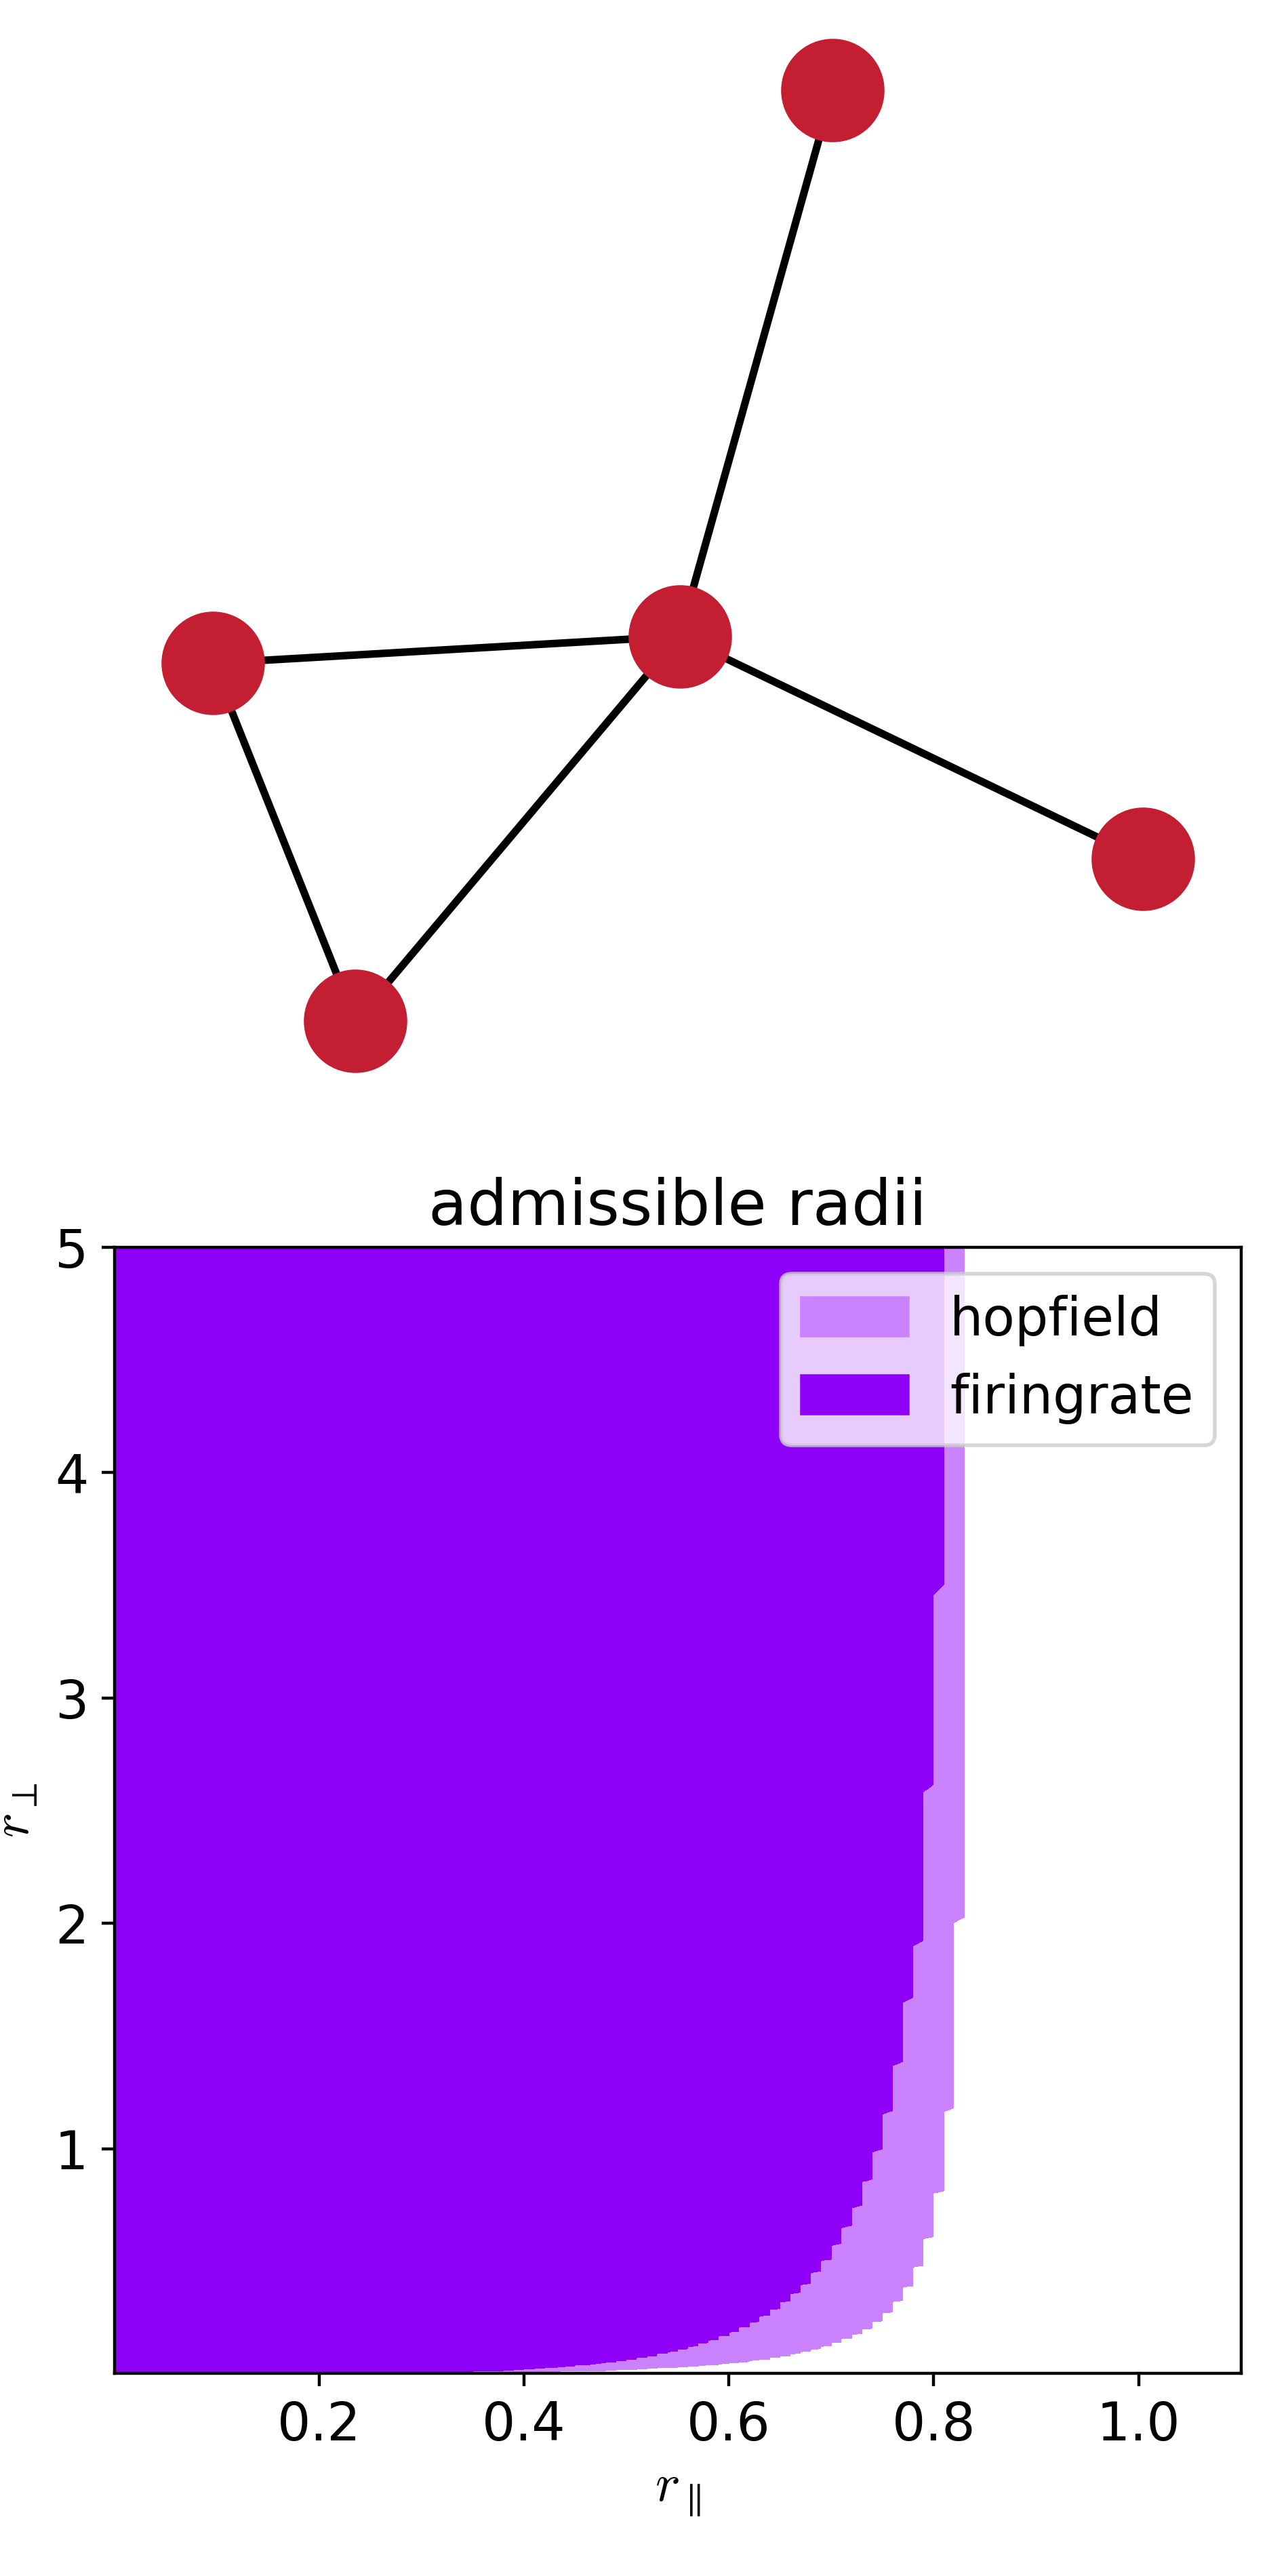
\includegraphics[height=55mm]{images/5_4.png}
        
        \column{0.32\textwidth}
        \centering
        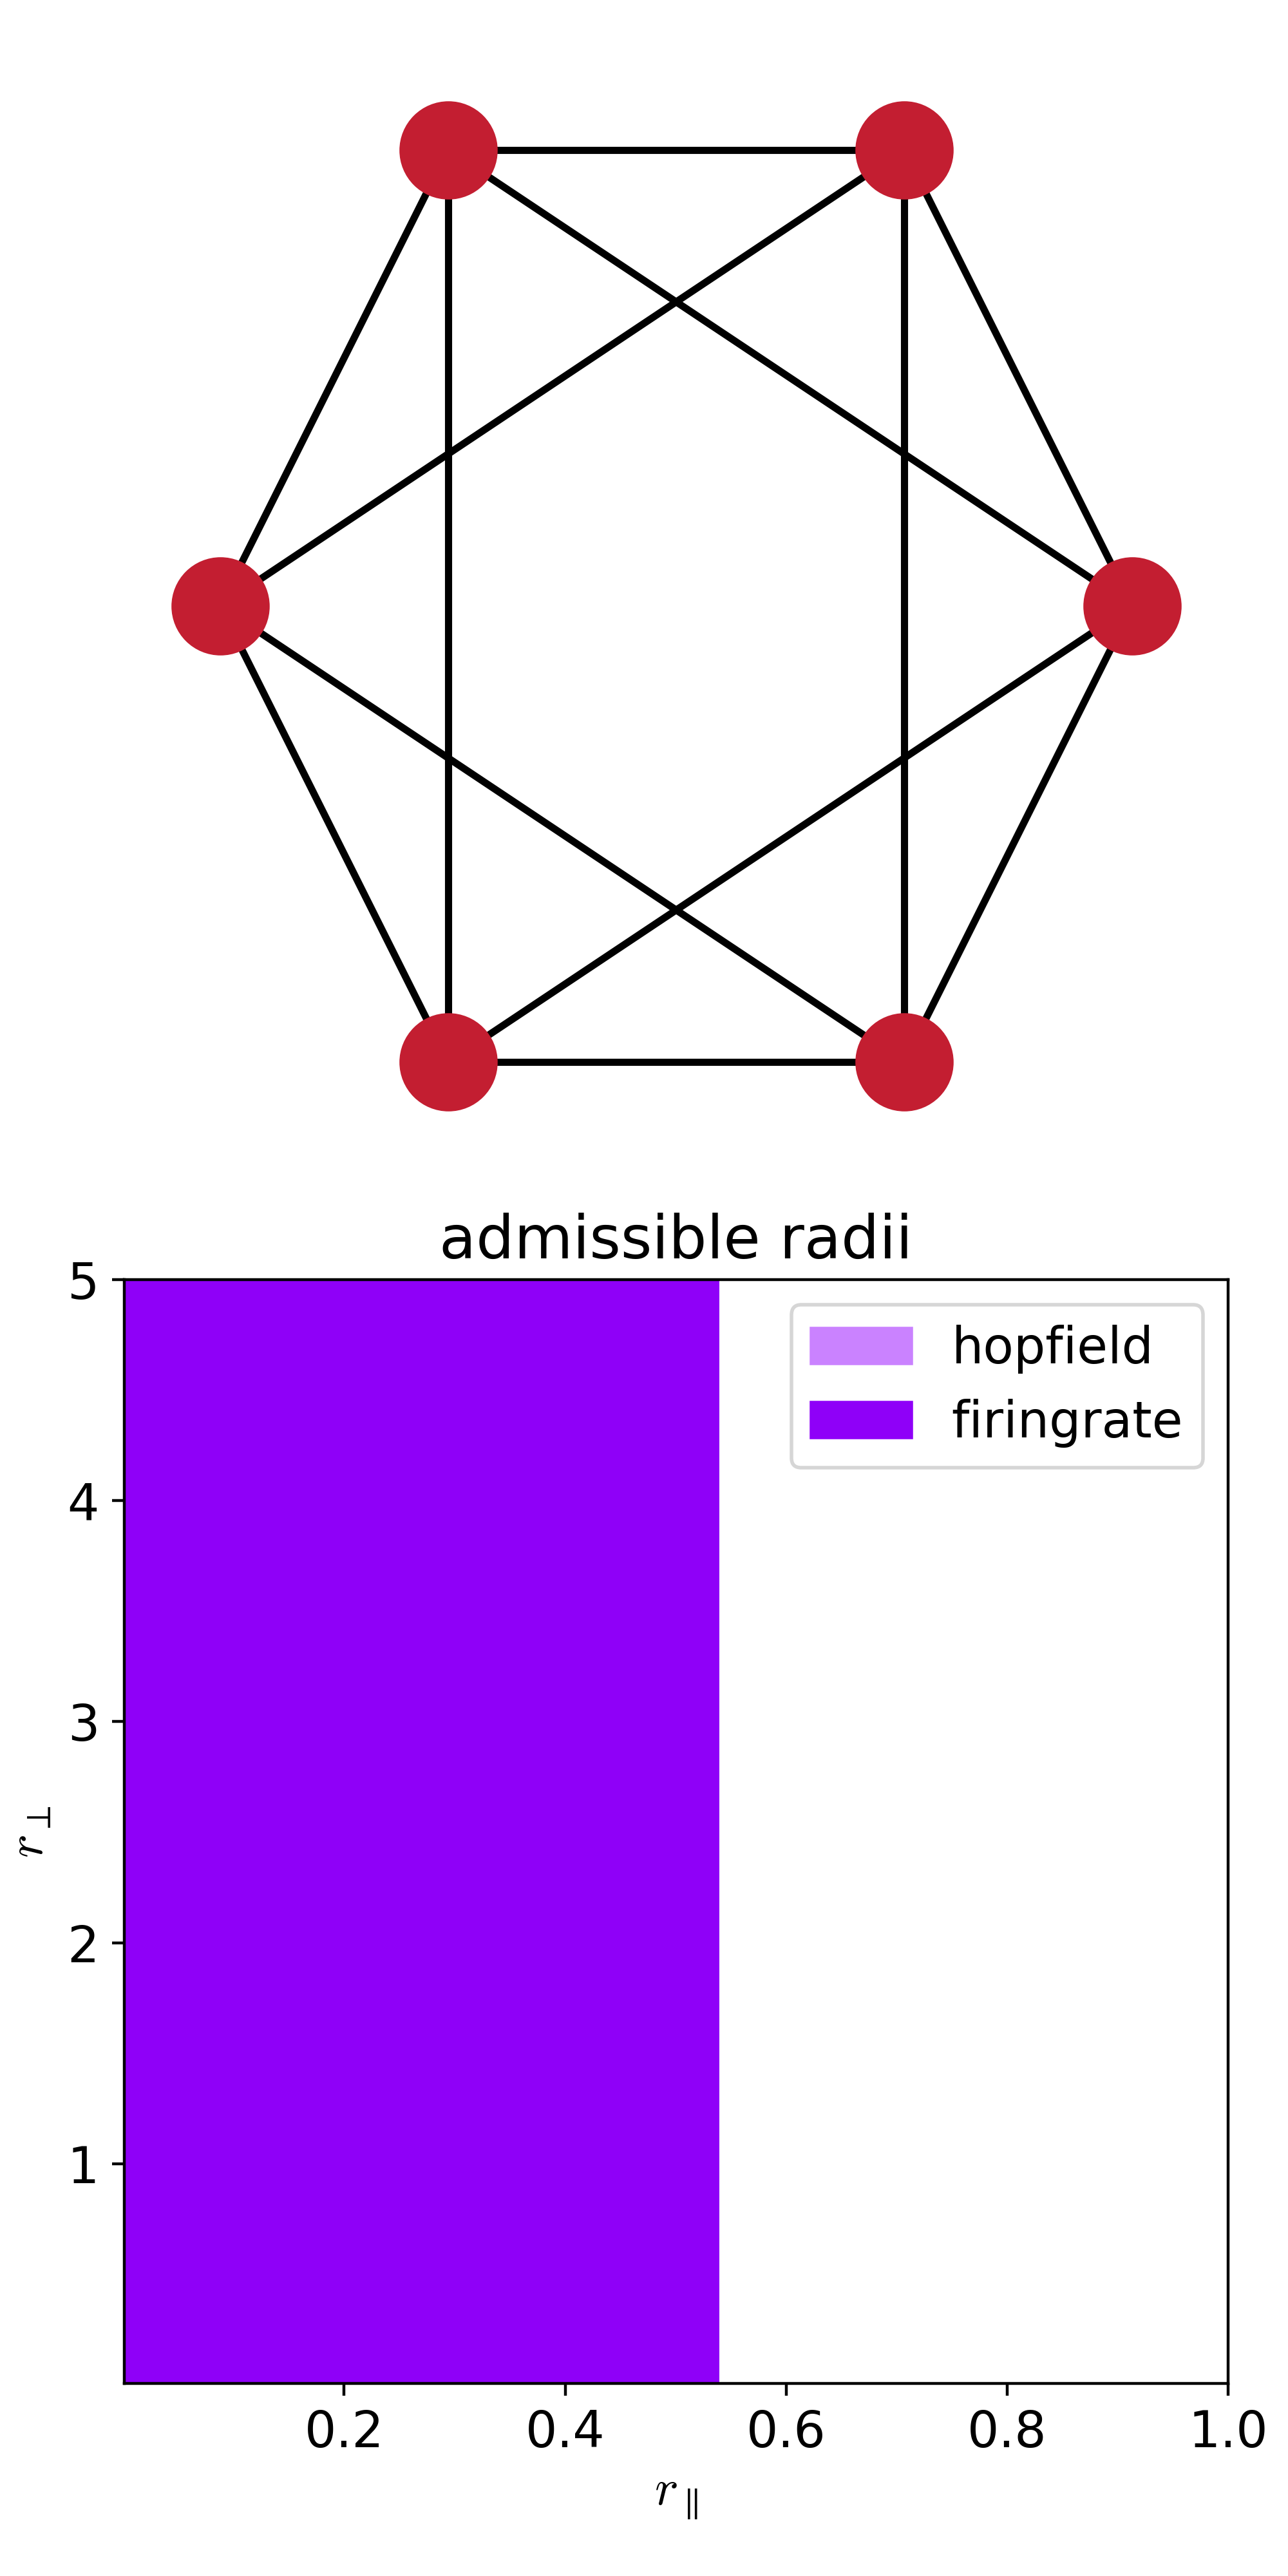
\includegraphics[height=55mm]{images/6_108.png}

        \column{0.32\textwidth}
        \centering
        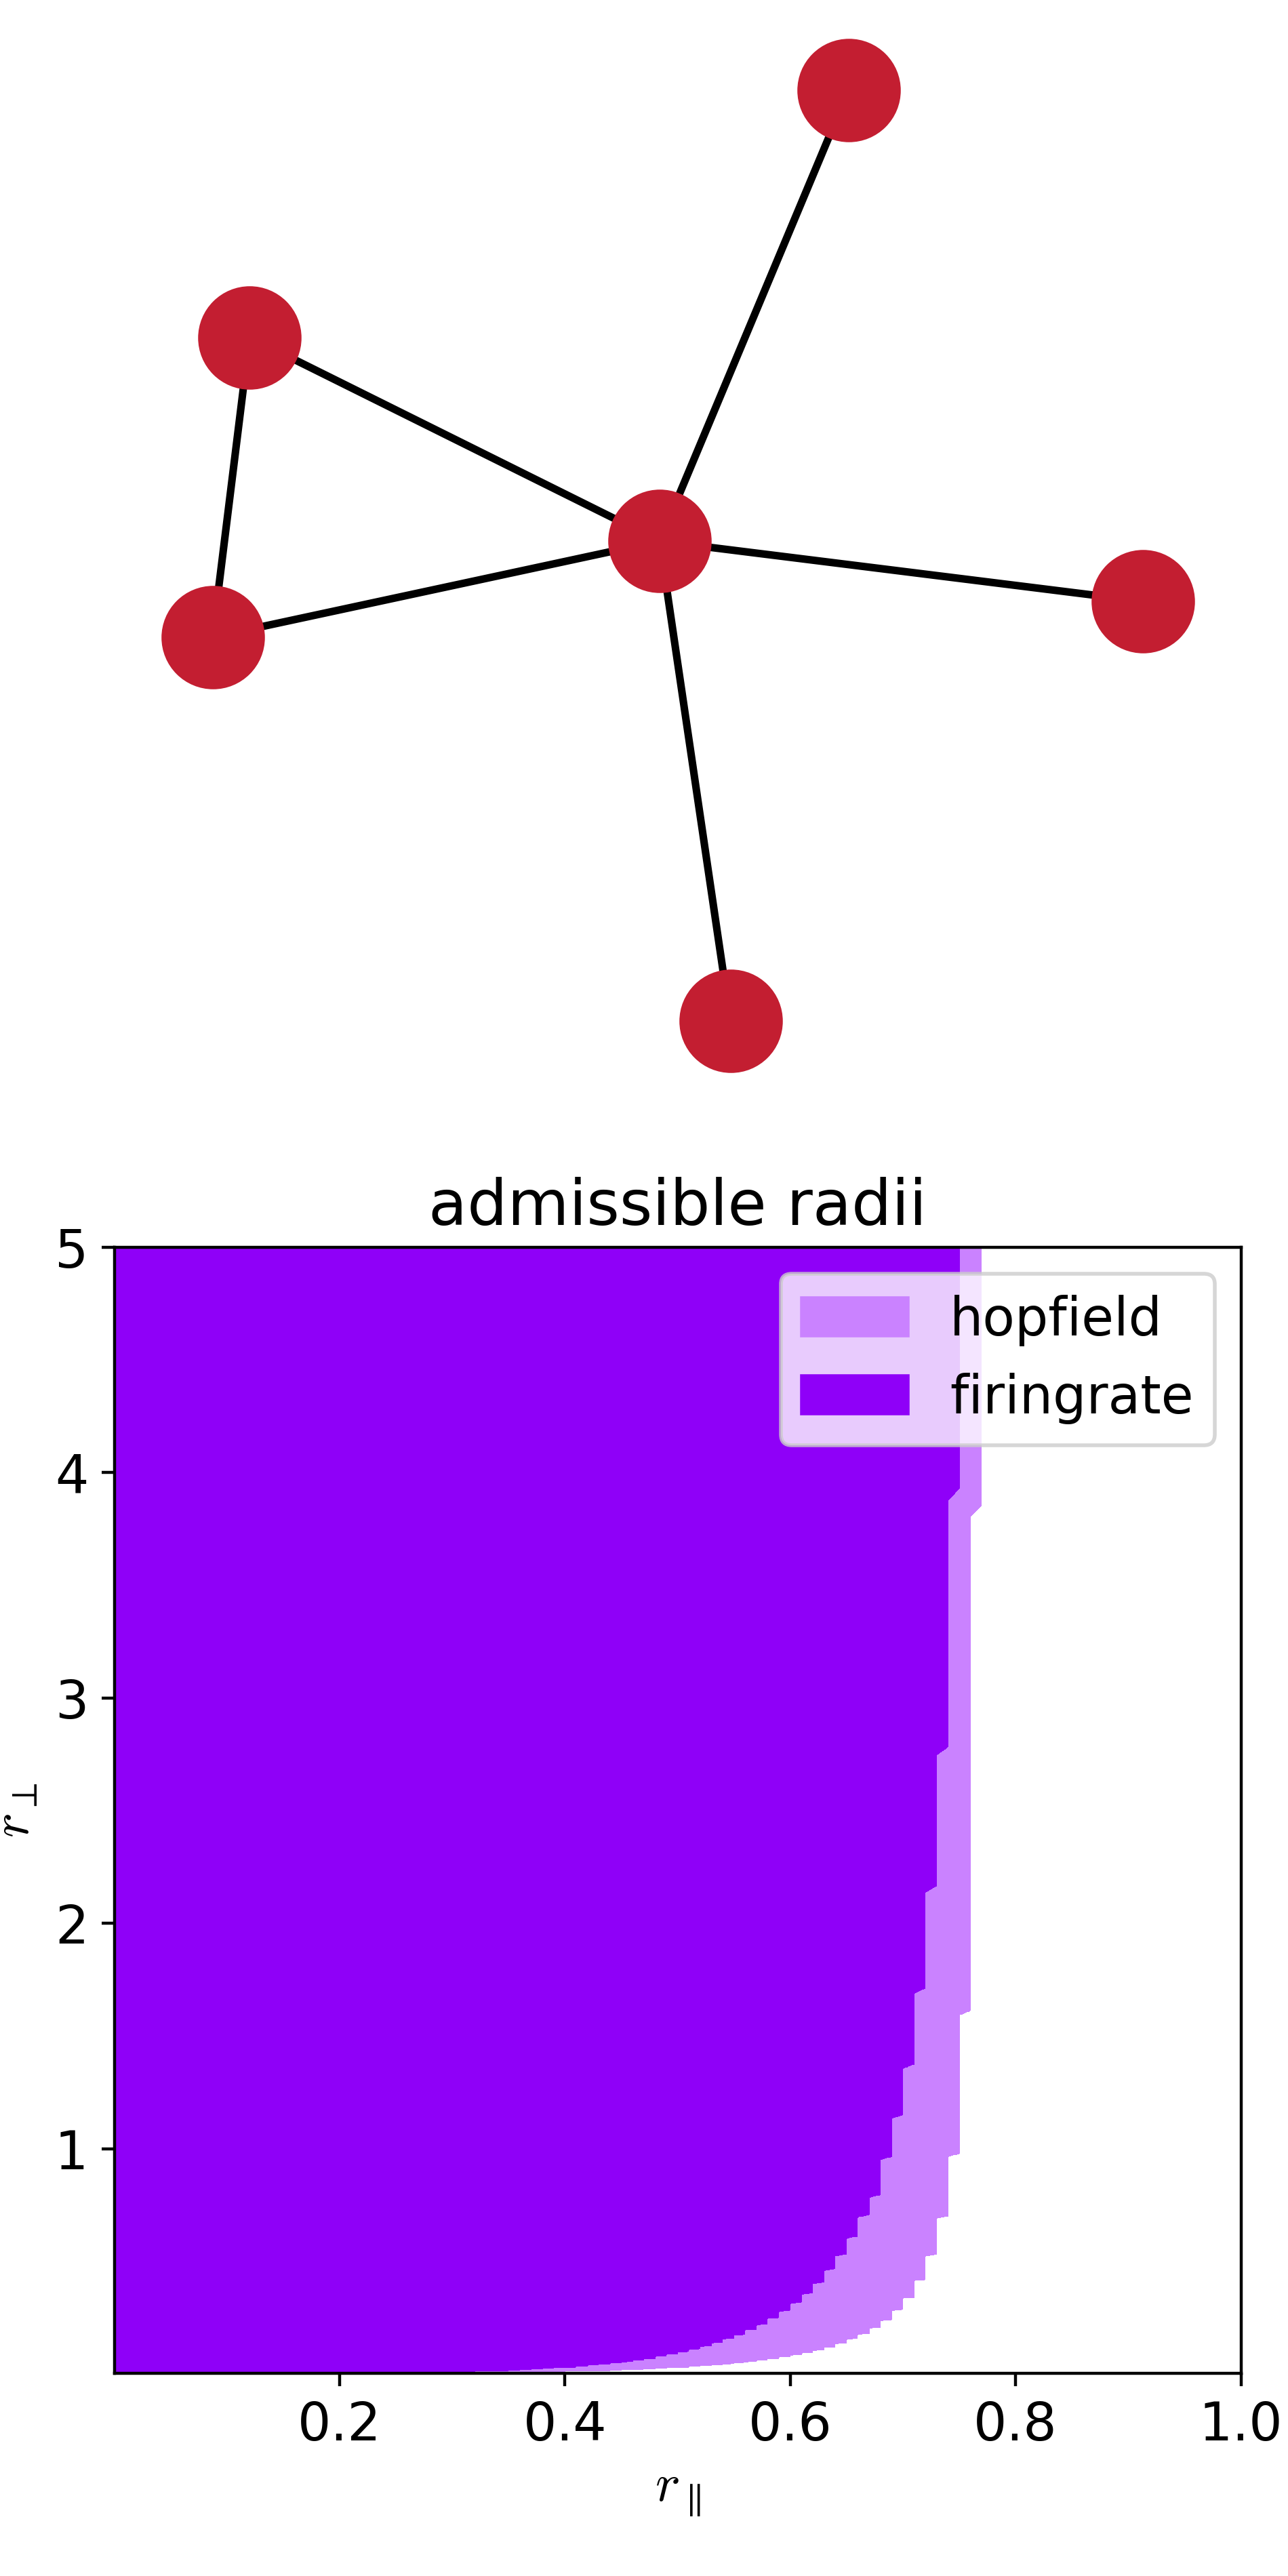
\includegraphics[height=55mm]{images/6_7.png}
    \end{columns}
    For arbitrary non-regular graph, bounds \(\rpr\) and \(\rpp\) are coupled, and the bounds for the Hopfield and Firing Rate cases need not be identical.
\end{frame}

\end{document}